\documentclass[11pt,aspectratio=1610,xcolor=dvipsnames]{beamer}

\usetheme[
    background=light,
    numbering=fraction,
    block=fill,
    progressbar=frametitle
]{metropolis}

\graphicspath{{img/}}

\usepackage[style=authortitle-ibid,backend=biber]{biblatex}
\addbibresource{refs.bib}
\setbeamerfont{footnote}{size=\scriptsize}

\usepackage{physics}
\usepackage{bbm}
\usepackage{booktabs}
\usepackage[most,skins,theorems]{tcolorbox}
\tcbset{variables/.style={colback=yellow!20,colframe=yellow}}
\usepackage{tikz}
\usetikzlibrary{shapes.geometric, arrows, shadows}
\usetikzlibrary{fit, backgrounds}



% \colorlet{LightLavender}{Lavender!40!}
\newtcolorbox{prob}{colback=red!5!white,colframe=red!75!black}
\usefonttheme[onlymath]{serif}
\usepackage{quantikz}
\usepackage{qrcode}
\usepackage{pgfplots}
\usepackage{pythonhighlight}

\newcommand{\R}{\mathbb{R}}
\newcommand{\U}[1]{\mathsf{U}(#1)}
\newcommand{\defeq}{\stackrel{\text{\tiny def}}{=}}

\titlegraphic{
\includegraphics[width=0.3\textwidth]{unitary_fund_logo.png}}

\title{Error Mitigation With Mitiq}
\subtitle{Coloquio de Cómputo Cuántico}
\date{Nov 29, 2022}
\author{Nate Stemen}

% \setbeamertemplate{frame footer}{N. Stemen: Unitary Fund}


\begin{document}

\maketitle

\begin{frame}{Overview}
	\begin{enumerate}
		\item Overview of Quantum Error Mitigation (QEM)
		      \begin{itemize}
			      \item Zero-Noise Extrapolation (ZNE)
			      \item Probabilistic Error Cancellation (PEC)
		      \end{itemize}
		\item Overview of Mitiq
		\item Unitary Fund
	\end{enumerate}
	\note{
		there will be time for questions at the end, but if there is something that needs more immediate clarification, please don't hesitate to interrupt
	}
\end{frame}

\begin{frame}{What is error mitigation?}
	\begin{center}
		\only<1->{
			\begin{quantikz}[row sep=0.3cm,column sep=0.3cm]
				& \gate{H} & \ctrl{1} & \ctrl{2} & \targ{}   & \qw       & \qw & \\
				& \qw      & \targ{}  & \qw      & \ctrl{-1} & \targ     & \qw & \qw \\
				& \qw      & \qw      & \targ{}  & \qw       & \ctrl{-1} & \qw &
			\end{quantikz}
		}
		\uncover<2->{
			$\longrightarrow$
			\begin{quantikz}[row sep=0.3cm,column sep=0.3cm]
				& \gate{H} & \ctrl{1} & \qw & \gate[3,style={starburst,fill=yellow,draw=red,line width=2pt,inner xsep=-4pt,inner ysep=-5pt}]{\text{noise}} & \ctrl{2} & \targ{}   & \qw       & \qw & \\
				& \qw      & \targ{}  & \qw &                                                                                                              & \qw      & \ctrl{-1} & \targ     & \qw & \qw \\
				& \qw      & \qw      & \qw &                                                                                                              & \targ{}  & \qw       & \ctrl{-1} & \qw &
			\end{quantikz}
		}
		\uncover<3->{
			$\longrightarrow$
			\begin{quantikz}[row sep=0.3cm,column sep=0.3cm]
				& \gate{H} & \ctrl{1} & \qw & \gate[2,style={starburst,fill=yellow!70,draw=red!50,line width=0.5pt,inner xsep=-7pt,inner ysep=-11pt}]{\text{noise}}  & \ctrl{2} & \targ{}   & \qw       & \qw & \\
				& \qw      & \targ{}  & \qw &                                                                                                                        & \qw      & \ctrl{-1} & \targ     & \qw & \qw \\
				& \qw      & \qw      & \qw & \qw                                                                                                                    & \targ{}  & \qw       & \ctrl{-1} & \qw &
			\end{quantikz}
		}
	\end{center}
\end{frame}

\begin{frame}{What about error correction?}
	\begin{figure}[h]
		\centering
		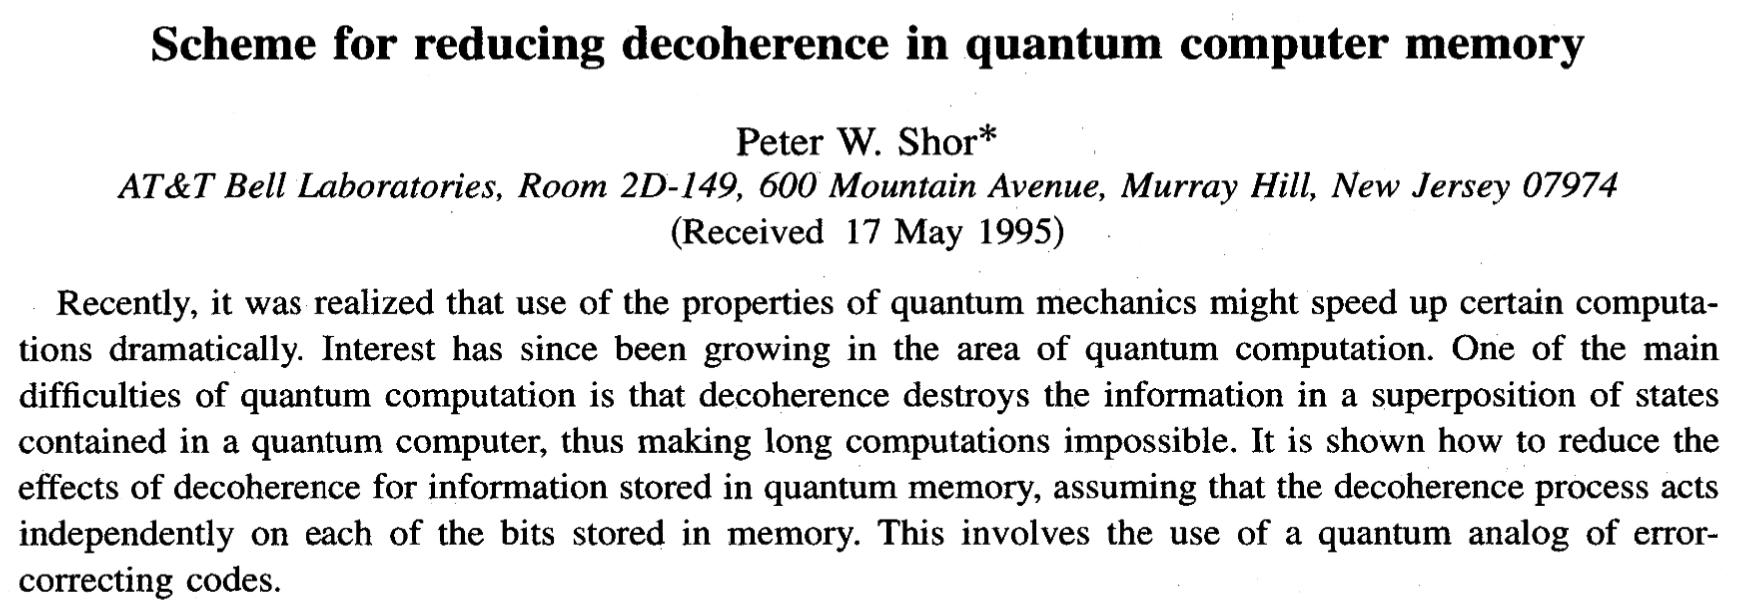
\includegraphics[width=.7\textwidth]{shor-qec.png}
		\note{first by shor, but also Steane and Calderbank in the years after refining the 9-qubit Shor code}
	\end{figure}
	\begin{columns}[t]
		\begin{column}{0.5\textwidth}
			\uncover<2->{
				\begin{block}{Error Correction}
					\begin{itemize}
						\item Encode logical qubits into many physical qubits
						\item Intermediate measurements produce syndromes
						\item Use syndromes to correct errors
					\end{itemize}
				\end{block}
			}
			\uncover<4->{
				\begin{tikzpicture}[overlay] % TODO: make transparent/change color
					\node[draw, fill=yellow, rotate=20, minimum width=5cm, minimum height=1cm] at (3.5, 2.5) {Scalable, but unfeasible};
				\end{tikzpicture}
			}
		\end{column}
		\begin{column}{0.5\textwidth}
			\uncover<3->{
				\begin{block}{Error Mitigation}
					\begin{itemize}
						\item Perform multiple and different noisy computations
						\item Collect results
						\item Infer ideal expectation values
					\end{itemize}
				\end{block}
			}
			\uncover<5->{
				\begin{tikzpicture}[overlay]
					\node[draw, fill=yellow, rotate=20, minimum width=5cm, minimum height=1cm] at (3.5, 1.95) {Unscalable$^*$, but feasible};
				\end{tikzpicture}
			}
		\end{column}
	\end{columns}
\end{frame}

\begin{frame}{QEM Methods}
	\begin{columns}[T]%,onlytextwidth]
		\begin{column}{0.33\textwidth}
			\begin{tcolorbox}[title=Zero-Noise Extrapolation,halign title=center,halign=center,colback=gray!20, colframe=gray!70]
				\vspace{-.5cm}
				\begin{equation*}
					\partial_t \rho = -i \comm{H}{\rho} + \lambda \mathcal{L}(\rho)
				\end{equation*}
			\end{tcolorbox}
			\begin{tcolorbox}[title=Symmetry-based techniques,halign title=center,halign=center,colback=gray!20, colframe=gray!70]
				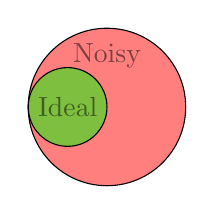
\begin{tikzpicture}
					\begin{scope}[fill opacity=0.5]
						\draw[fill=red, draw = black] (0,0) circle (1);
						\draw[fill=green, draw = black] (-.5,0) circle (.5);
						\node at (0,0.65) (A) {Noisy};
						\node at (-.5,0) (B) {Ideal};
					\end{scope}
				\end{tikzpicture}
				\vspace{-.5cm}
				\begin{align*}
					M \ket{\psi} & = \ket{\psi}                  \\
					\rho         & = \frac{M \rho M}{\tr(M\rho)}
				\end{align*}
			\end{tcolorbox}
		\end{column}
		\begin{column}{0.33\textwidth}
			\begin{tcolorbox}[title=Probabilistic Error Cancellation,halign title=center,halign=center,colback=gray!20, colframe=gray!70]
				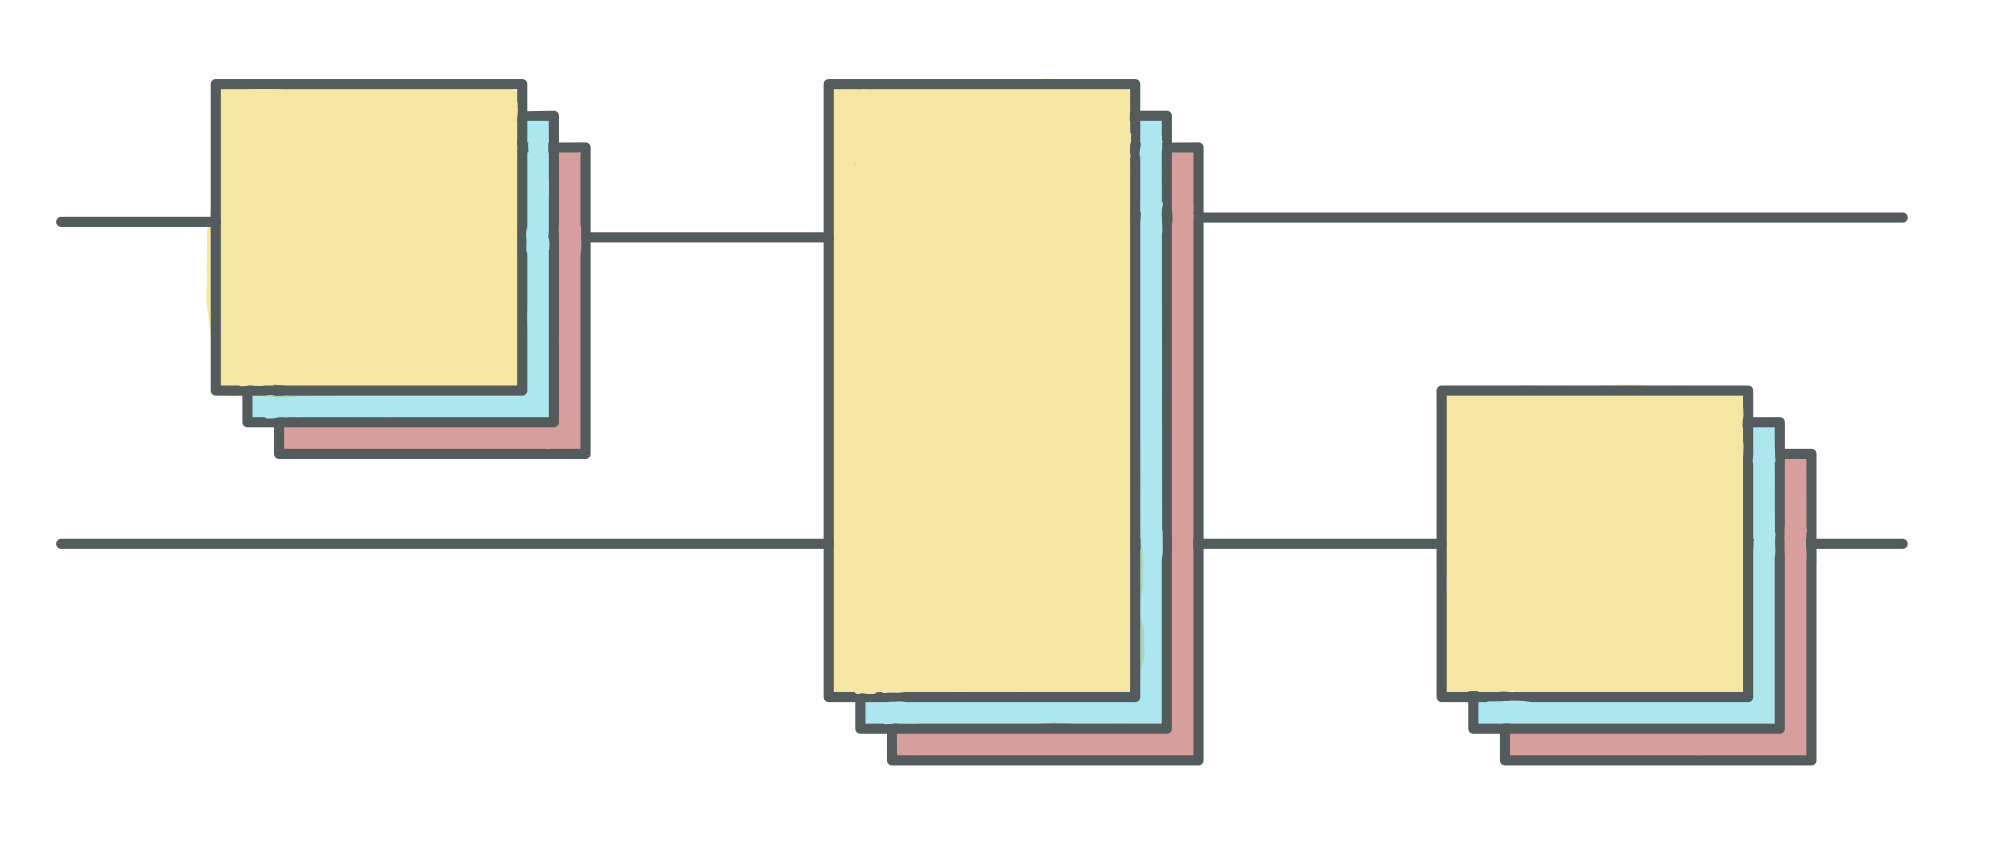
\includegraphics[width=\textwidth]{peccircuits.jpeg}
			\end{tcolorbox}
			\begin{tcolorbox}[title=Dynamical Decoupling/Randomized Compiling,halign title=center,halign=center,colback=gray!20, colframe=gray!70]
				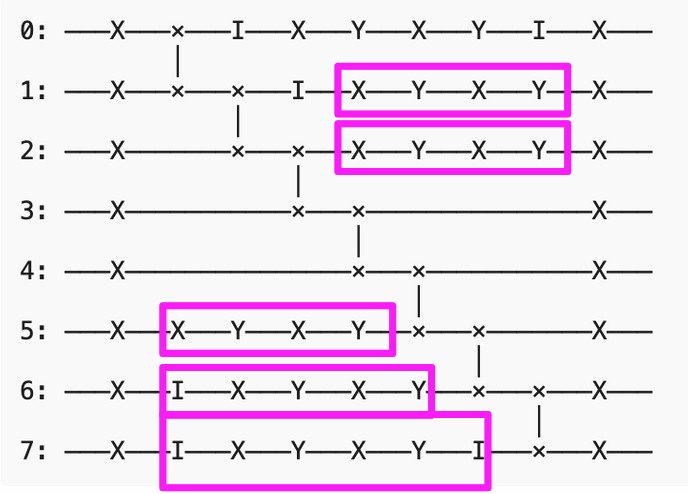
\includegraphics[width=\textwidth]{dd.png}
			\end{tcolorbox}
		\end{column}
		\begin{column}{0.33\textwidth}
			\begin{tcolorbox}[title=Learning-based methods,halign title=center,halign=center,colback=gray!20, colframe=gray!70]
				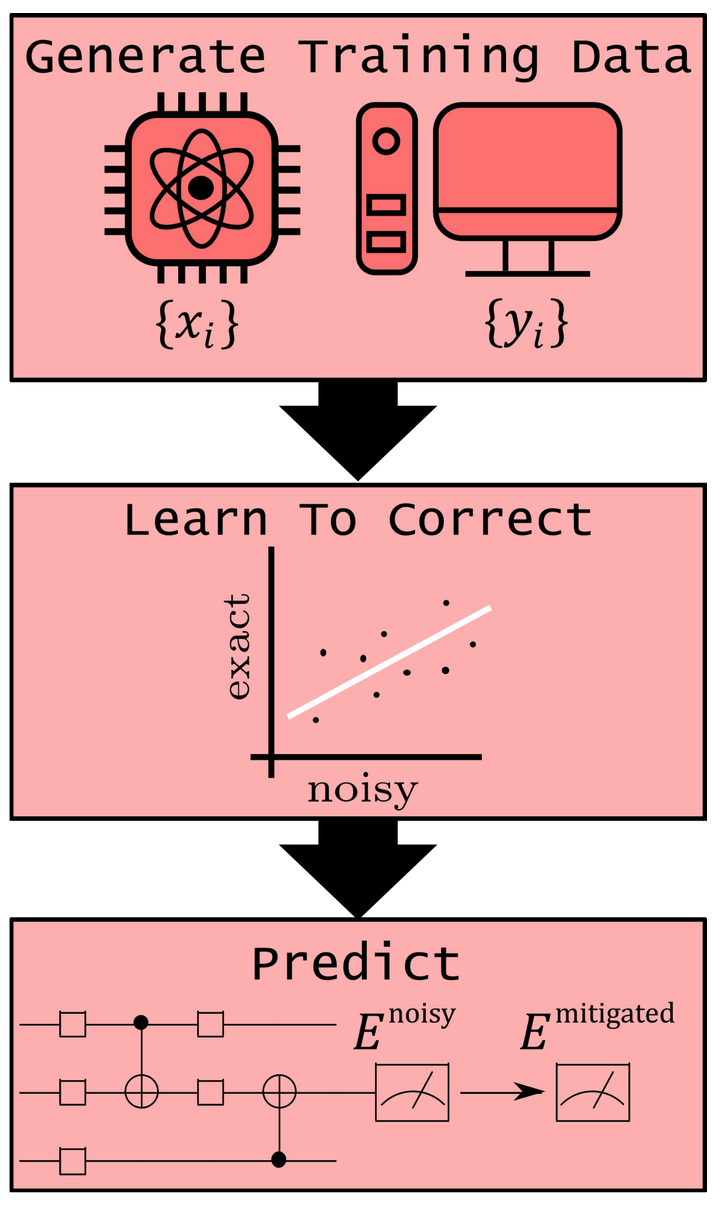
\includegraphics[width=\textwidth]{learning-based.png}
			\end{tcolorbox}

		\end{column}
	\end{columns}

\end{frame}

\begin{frame}{Zero-Noise Extrapolation (ZNE)}

	\begin{exampleblock}{Key Idea}
		Scale noise up, extrapolate back to zero-noise value.
	\end{exampleblock}

	\begin{columns}
		\begin{column}{0.4\textwidth}
			\uncover<2->{
				\vspace{-2cm}
				\begin{equation*}
					\partial_t \rho = - i \comm{H}{\rho} + \lambda \mathcal{L}(\rho)
				\end{equation*}
			}
			\vspace{-1cm}
			\uncover<3->{
				\begin{center}
					\begin{tikzpicture}% TODO: add drawing for later slides
						\draw[very thin,color=gray] (-0.1,-0.1) grid [xstep=1.5] (4.9, 3.9);

						\draw[->] (-0.2,0) -- (5.2,0) node[below] {$\lambda$};
						\draw[->] (0,-0.2) -- (0,4.2) node[left] {$\expval{A}_\lambda$};
					\end{tikzpicture}
				\end{center}
			}
		\end{column}

		\begin{column}{0.6\textwidth}
			\uncover<4->{How do we scale the noise \textbf{up}?}
			\uncover<5->{
				\begin{center}
					\begin{tikzpicture}
						\begin{axis}[ymin=0, ymax=10, xmin=-.5, xmax=16.5, tiny, axis y line=left, ytick=\empty, axis x line=bottom, xtick=\empty, xlabel=$t$]
							\addplot[blue, ultra thick] table {pulse.dat};
						\end{axis}
					\end{tikzpicture}%
					\quad
					\begin{tikzpicture}
						\begin{axis}[x=.25cm, ymin=0, ymax=10, xmin=-.5, xmax=16.5, tiny, axis y line=left, ytick=\empty, axis x line=bottom, xtick=\empty, xlabel=$t$]
							\addplot[blue, ultra thick] table {pulse.dat};
						\end{axis}
					\end{tikzpicture}%
				\end{center}
			}
			\begin{columns}[onlytextwidth]
				\begin{column}{0.5\textwidth}
					\vspace{3cm}
					\uncover<6->{
						\begin{quantikz}
							& \gate{} & \gate[2]{}  & \qw     & \qw \\
							& \qw     &             & \gate{} & \qw
						\end{quantikz}
					}
				\end{column}
				\begin{column}[t]{0.5\textwidth}
					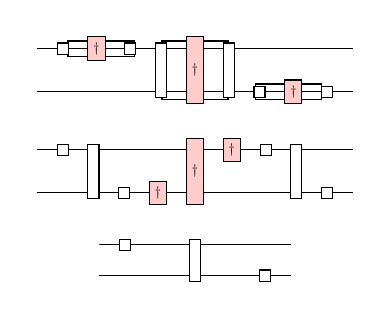
\begin{tikzpicture}
						\uncover<6-6>{
							\node[scale=.7] {
								\begin{quantikz}
									& \gate[][1.2cm]{} & \gate[2][1.2cm]{} & \qw              & \qw \\
									& \qw              &                   & \gate[][1.2cm]{} & \qw
								\end{quantikz}
							};
						}
						\uncover<7->{
							\node[scale=.5] (local) {
								\begin{quantikz}
									& \gate{} & \gate[style={fill=red!20}]{\dagger} & \gate{} & \gate[2]{} & \gate[2, style={fill=red!20}]{\dagger} & \gate[2]{} & \qw     & \qw                          & \qw     & \qw \\
									& \qw     & \qw                          & \qw     &            &                                 &            & \gate{} & \gate[style={fill=red!20}]{\dagger} & \gate{} & \qw
								\end{quantikz}
							};
							\node[scale=.5, below=.2cm of local] (global) {
								\begin{quantikz}
									& \gate{} & \gate[2]{}  & \qw     & \qw     & \gate[2, style={fill=red!20}]{\dagger} & \gate[style={fill=red!20}]{\dagger} & \gate{} & \gate[2]{}  & \qw     & \qw \\
									& \qw     &             & \gate{} & \gate[style={fill=red!20}]{\dagger} &            & \qw     & \qw     &             & \gate{} & \qw
								\end{quantikz}
							};
							\node[scale=.5, below=.2cm of global] (ii) {
								\begin{quantikz}
									& \gate{} & \qw & \qw & \gate[2]{} & \qw & \qw & \qw     & \qw \\
									& \qw     & \qw & \qw &            & \qw & \qw & \gate{} & \qw
								\end{quantikz}
							};
						}
					\end{tikzpicture}
				\end{column}
			\end{columns}
		\end{column}
	\end{columns}
\end{frame}

\begin{frame}[t]{Probabilistic Error Cancellation (PEC)}
	\begin{exampleblock}{Key Idea}
		Use noisy operations to build up noiseless ones by selective cancellation and sampling.
	\end{exampleblock}

	\begin{columns}[t]
		\begin{column}{0.5\textwidth}
			\uncover<3->{
				\begin{center}
					\begin{quantikz}
						& \gate{} & \gate[2]{}  & \qw     & \qw \\
						& \qw     &             & \gate{} & \qw
					\end{quantikz}

					$\downarrow$
				\end{center}
				\vspace{-0.5cm}
				\begin{figure}[h]
					\centering
					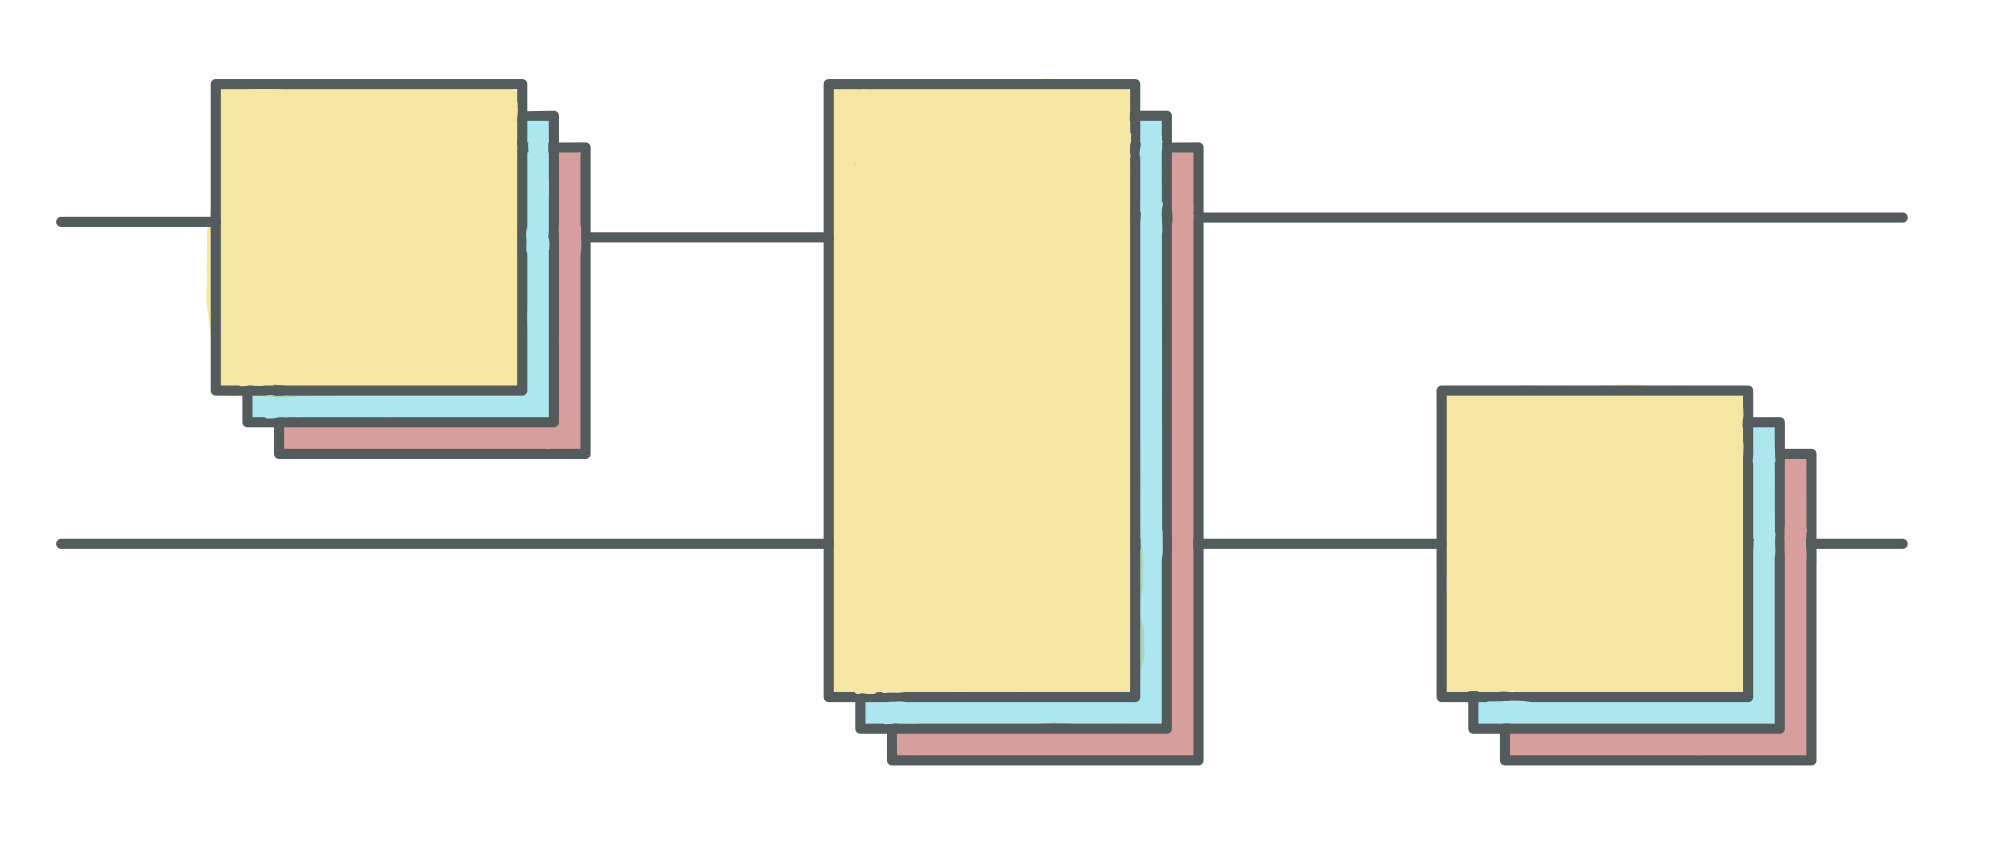
\includegraphics[width=0.9\textwidth]{peccircuits.jpeg}
				\end{figure}
			}
		\end{column}
		\begin{column}{0.5\textwidth}
			\uncover<2->{% TODO: show this sooner
				\begin{equation*}
					\mathcal{U} = \sum_{i = 1}^n a_i \mathcal{O}_i
				\end{equation*}
			}
			\uncover<4->{
				\begin{equation*}
					\expval{A}_\text{PEC} = \frac{\gamma}{M}\sum_{i = 1}^M \sigma_i \expval{A}_i
				\end{equation*}
			}

			\uncover<2->{
				\begin{tcolorbox}[variables]
					\uncover<2->{- $\mathcal{O}_i$: implementable operations}

					\uncover<4->{
						- $\sigma_i$: Sign of $i^\text{th}$ circuit

						- $M$: \# of circuits

						- $\gamma$: overall negativity (product of representation one-norms)
					}
				\end{tcolorbox}
			}
		\end{column}
	\end{columns}
\end{frame}


\tikzset{rect/.style={rectangle, rounded corners, minimum width=3.5cm,
			minimum height=1cm, text centered, draw=Cerulean!50, fill=Cerulean!10},
	arrow/.style={thick,->,>=stealth}}
\begin{frame}{Running quantum programs in practice}
	\begin{center}
		\begin{tikzpicture}%[node distance=2cm]

			\node (qp) [rect] {Quantum Program};
			\node (backend) [rect, right = 1cm of qp] {Execute};
			\node (result) [rect, below = 1.50cm  of qp] {Results};

			\draw [arrow] (qp) -- (backend);
			\draw [arrow] (backend) |- (result);
			\coordinate (aux) at (result.south -| backend);
			\coordinate (aux2) at (qp.north -| backend);

			\begin{scope}[on background layer]
				\node[draw, dashed, gray, rounded corners, fill=red!20, fit=(qp) (result), label={above:User}]{};
				\node[draw, dashed, gray, rounded corners, fill=gray!50, fit=(backend) (aux) (aux2), label={above:Hardware/Simulator}]{};
			\end{scope}
		\end{tikzpicture}
	\end{center}
\end{frame}

\begin{frame}{Running quantum programs in practice with Mitiq}
	\begin{center}
		\begin{tikzpicture}%[node distance=2cm]

			\node (qp) [rect] {Quantum Program};

			\node (many) [rect, below right = -0.8cm and .7cm of qp] {};
			\node [rect, below right = -0.9cm and .6cm of qp] {};
			\node (circuits) [rect, right = .5cm of qp] {Intermediary circuits};

			\node (backend) [rect, right = .7cm of circuits] {Execute};

			\node [rect, below left = 1.3cm and .5cm of backend] {};
			\node [rect, below left = 1.4cm and .6cm of backend] {};
			\node (noisy) [rect, below left = 1.5cm and .7cm of backend] {Noisy results};

			\node (result) [rect, below = 1.50cm  of qp] {Results};

			\draw [arrow] (qp) -- (circuits);
			\draw [arrow] (circuits) -- (backend);
			\draw [arrow] (backend) |- (noisy);
			\draw [arrow] (noisy) -- (result);
			\coordinate (aux) at (result.south -| backend);
			\coordinate (aux2) at (qp.north -| backend);

			\begin{scope}[on background layer]
				\node[draw, dashed, gray, rounded corners, fill=red!20, fit=(qp) (result), label={above:User}]{};
				\node[draw, dashed, gray, rounded corners, fill=gray!50, fit=(backend) (aux) (aux2), label={above:Hardware/Simulator}]{};
				\node[draw, dashed, gray, rounded corners, fill=yellow!50, fit=(circuits) (many) (noisy), label={above:Error Mitigation}]{};
			\end{scope}
		\end{tikzpicture}
	\end{center}
\end{frame}

\begin{frame}{Mitiq: Demo!}
	\begin{center}
		\url{https://mitiq.readthedocs.io/}

		\qrcode{https://mitiq.readthedocs.io/}
	\end{center}
\end{frame}

\begin{frame}{Does it work?}
	\begin{figure}[h]
		\centering
		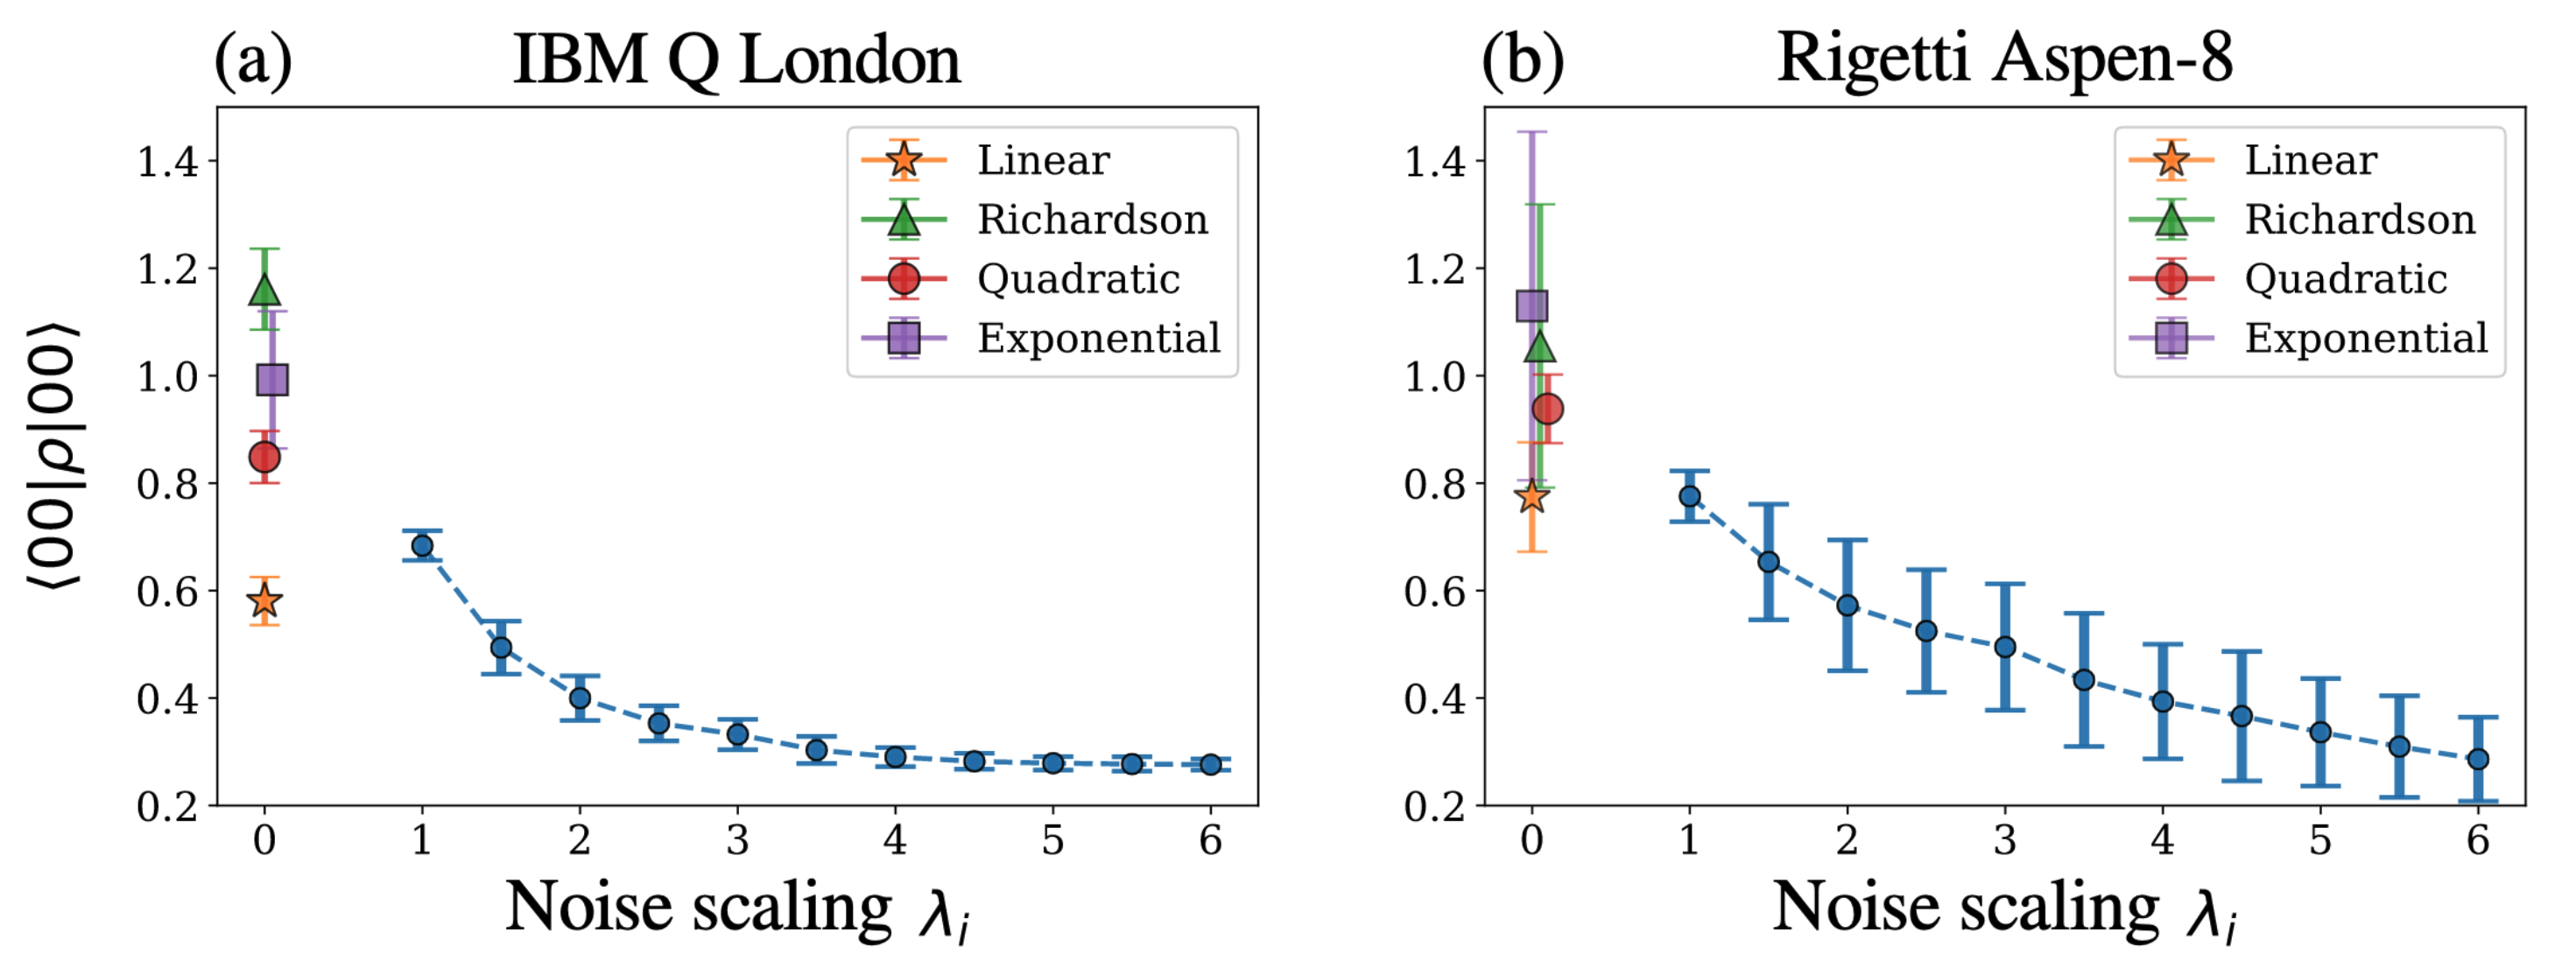
\includegraphics[width=\textwidth]{results.png}
	\end{figure}
	\hfill Quantum 6, 774 (2022). \qrcode[height=1.4cm]{https://quantum-journal.org/papers/q-2022-08-11-774/}
\end{frame}

\begin{frame}{Unitary Fund}
	\begin{columns}
		\begin{column}{0.5\textwidth}
			\only<1-1>{
				\begin{figure}[h]
					\centering
					
\includegraphics[width=\textwidth]{team.png}
				\end{figure}
			}
			\only<2-2>{
				Microgrant Program:
				\begin{itemize}
					\item 68 Microgrants awarded
					\item 23 countries
					\item 16+ publications
					\item 30+ libraries, \~6k commits
					\item 2 startups, 2 nonprofit
				\end{itemize}
			}
			\only<4-4>{
				\begin{figure}[h]
					\centering
					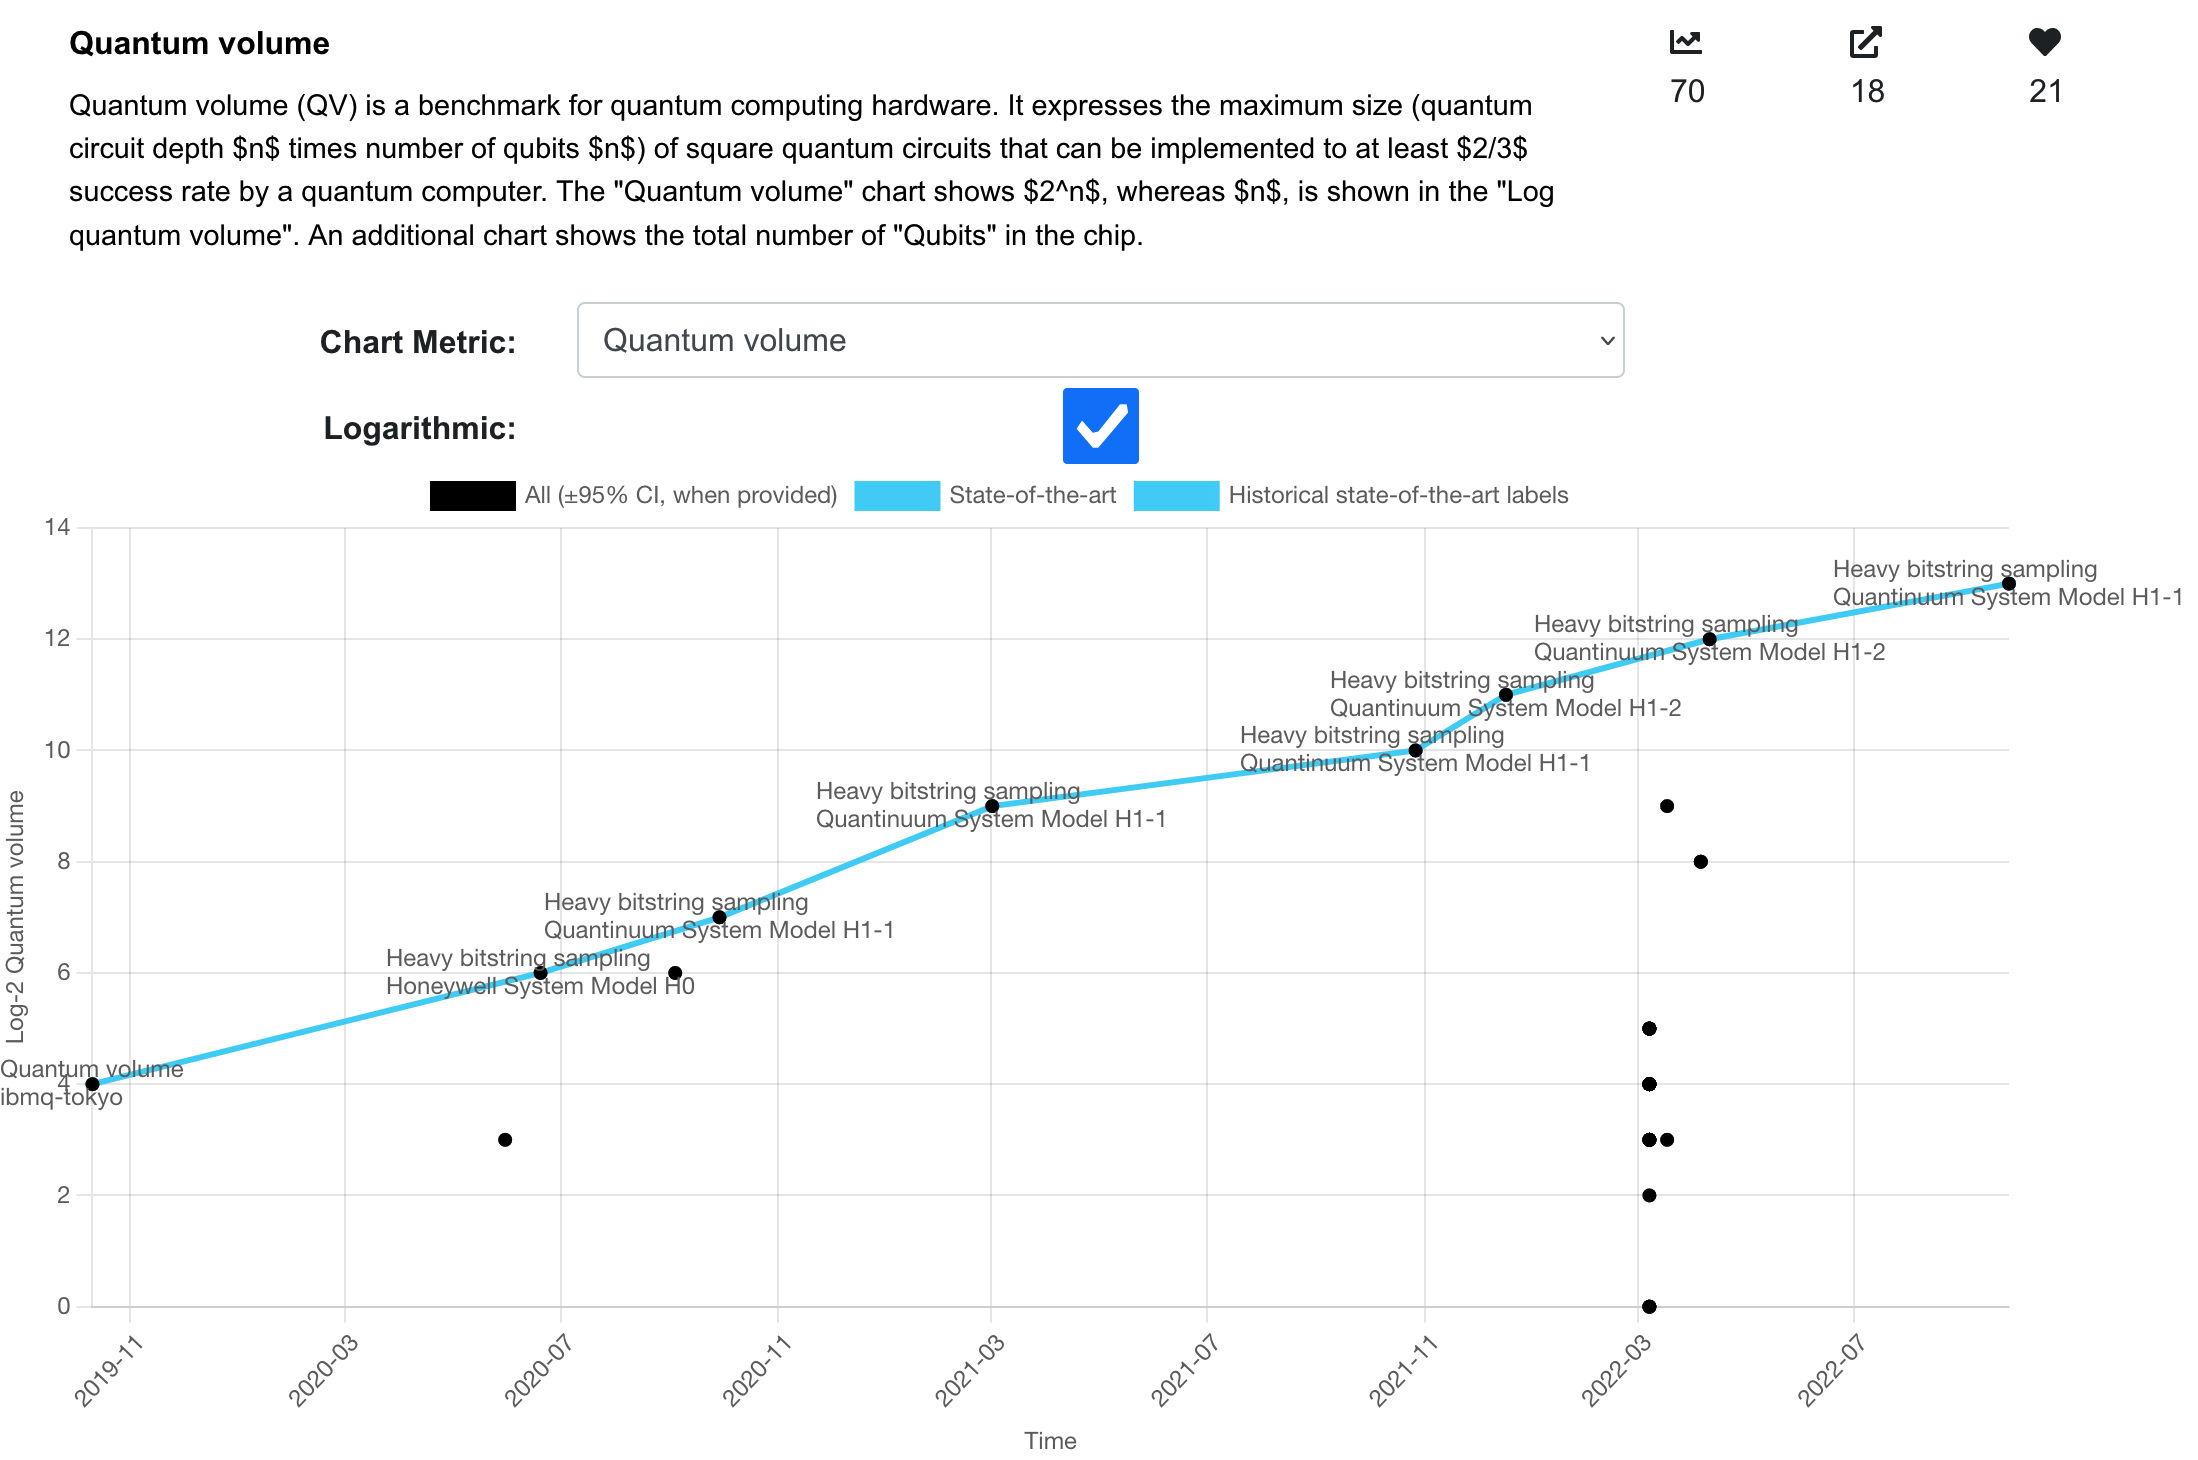
\includegraphics[width=1.1\textwidth]{metriq-web.png}
					\url{https://metriq.info}
				\end{figure}
			}
			\only<5-5>{
				\begin{itemize}
					\item UnitaryHACK
					      \begin{itemize}
						      \item 30 participating projects
						      \item 66 bounties (with cash prizes)
						      \item Look out for news on UnitaryHACK 2023!
					      \end{itemize}
					\item \url{http://discord.unitary.fund}
					      \begin{itemize}
						      \item Community calls for projects: Mitiq, QIR Alliance, QuTiP, OpenQAOA
					      \end{itemize}
				\end{itemize}
				\begin{center}
					\qrcode[height=1.5cm]{http://discord.unitary.fund}
				\end{center}
			}

		\end{column}
		\begin{column}{0.5\textwidth}
			\begin{itemize}[<+->]
				\item 501(c)(3) nonprofit dedicated to growing the quantum open-source ecosystem
				\item \alert<2>{Run microgrant program; \$4k grants to those developing cool quantum projects in the open}
				\item Develop 
\includegraphics[width=0.25\textwidth]{mitiq-logo.png}
				\item \alert<4>{Run 
\includegraphics[width=0.25\textwidth]{metriq-logo.png} (\url{metriq.info}): a platform for community driving quantum benchmarks}
				\item \alert<5>{Community development}
			\end{itemize}
		\end{column}
	\end{columns}
\end{frame}

\setbeamercovered{transparent}

\begin{frame}{Summary}
	\begin{itemize}
		\item QEM is a growing field of research working towards better results for existing quantum computers.
		\item ZNE and PEC are promising, and easy to use techniques.
		\item Mitiq can provide out-of-the-box support for running quantum programs with QEM.
		\item Unitary Fund is helping grow the quantum open-source community and ecosystem.
	\end{itemize}
\end{frame}

% \begin{frame}{References}
% 	\nocite{*}
% 	\printbibliography[heading=none]
% \end{frame}

\begin{frame}[standout]
	Thank you!
\end{frame}

\end{document}
